\chapter{Results}

The Artefact that was created in Chapter \ref{ch3} could identify StyleGAN images with very high accuracy. The various results achieved in the development of the Artefact will be discussed and evaluated. The initial neural network accuracy will be discussed and example output from the artefact making the predictions will be demonstrated. The hyperparameter optimized neural network that acts as this project final model will be compared to the initial model and the model created by \cite{Wang} to demonstrate the large gains made to the model performance using optimization in constrained resources environment. 

\section{The First Neural Network}

The neural network created in Sprint 1 produced a detection accuracy of 61\% by just replacing StyleGAN generated and real human images with the Cat-vs-Dog images in the introduction to CNN's exercise. The accuracy achieved acted as a proof of concept. Using Hot and Cold learning techniques improved the model to a training accuracy of 81\%. When testing the improvements made in hot and cold learning the real accuracy that the model identifies StyleGAn images was 69\%, which means the model still cannot extract features from the images in the dataset but can generalize some features. The relatively high accuracy of the simplest implementation and the increase in accuracy when applying hot and cold learning shows how powerful CNN's can be in a world with increasing artificially generated images. 

Figure \ref{fig:reswrong} shows the self-created model implemented in the front-end artefact predicting on StyleGAN images and real human images from the FlickrFaces dataset. Although the model's prediction confidence is low, the prediction is advantageous compared to a random guess. A random guess and a neural network accuracy of 50\% can be seen as providing the same value. If a model predicts with only 50\% accuracy then code that mimics a coin flip prediction by random selection will provide the same results to the user. Therefore with the first neural network model starting with an accuracy higher than 60\% and the then reworked model providing an accuracy of 69\% was the value added by this project successful from the first iteration of the artefact development. Figure \ref{fig:reswrong} below shows the initial models deficiencies when identifying StyleGAN images.

\begin{figure}[H]%
\centering
\fbox{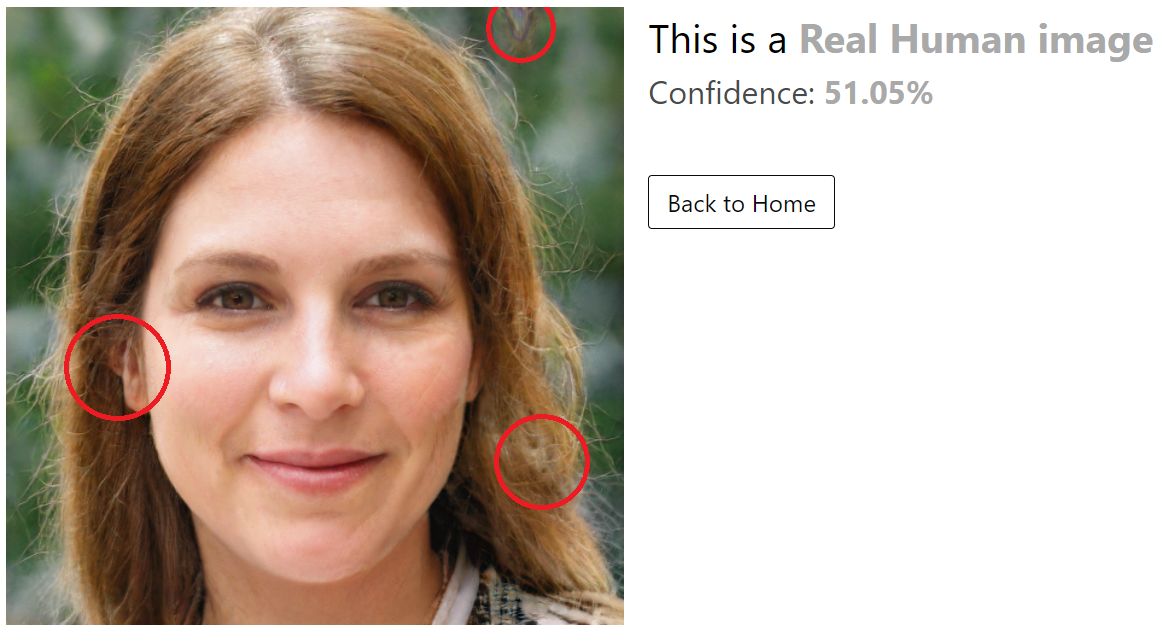
\includegraphics[width=0.95\textwidth]{img/fwrong.png}}%
\caption{Incorrect prediction from the initial model}%
\label{fig:reswrong}%
\end{figure}

Figure \ref{fig:reswrong}  and Table \ref{tabl:res1} shows the neural network that was created based on the activities in the 1st Sprint and concluded in the second sprint using hot and cold learning. The model correctly predicts most human images it receives but struggles with identifying StyleGAN images. What was obtained from this real image tending accuracy is that in the event of a StyleGAN prediction the user can be sure that the image has counter fitting properties, in this problem that would be StyleGAN artefact. That means that this model can be used in practice but only to a certain extent and cannot provide strong assurance. The results in Table \ref{tabl:res1} further illustrates the model's accuracy with real human images and its struggle with StyleGAN generated images.

\begin{table}[H]%
\caption{Real Images detected vs StyleGAN images detected in the initial model}
\label{tabl:res1}
\centering
\large
%\resizebox{0.60\textwidth}{!}{
\begin{tabular}{cccc}
\hline
Type of Image & & & Identification Accuracy  \\ 
\hline
StyleGAN & & & 68.00\% \\
Real Human & & & 77.20\% \\
\hline
\end{tabular}

\end{table} 

The misclassification of the initial model can partly be due to it not being optimized and therefore missing fine features in StyleGAN images. Some generalization occurred in this model and thus the results of the accuracy in SyleGAN misclassification echoed into the results of Real Human detection with high accuracy.

\section{The Optimized model}

The final model that was created in Sprint 3 improved in accuracy drastically. The model compared to the previous model is shown in Table below and a clear gain inaccuracy can be seen. The optimized model improved to such a high level of feature recognition in the StyleGAN data that the model's prediction on StyleGAN2 generated images is similar to the 1\textsuperscript{st} model created in the artefact developments prediction on StyleGAN1 images. Optuna greatly improved to model to such a high accuracy level in StyleGAN1 models that the model can contend with the model created by \cite{Wang} for the identification of CNN images. If using only StyleGAN1 images the model that was created for the artefact of this project is as effective as the model created by \cite{Wang}. The improvement that was made on the process for the model created in this project is the less restraining training and requirements for resources.

\begin{table}[H]%
\caption{Model comparison in terms of Accuracy and Confidence}
\label{tabl:res2}
\centering
\large
%\resizebox{0.60\textwidth}{!}{
\begin{tabular}{cccc}
\hline
Created Models & & Tested Accuracy  & Average Confidence\\ 
\hline
Cat-vs-Dog replacement & & 61.00\% & 57.00\%\\
Hot and Cold learning & & 69.00\% & 65,37\%\\
Hyperparameter Optimized & & 97,60\% & 96,98\%\\
\hline
\end{tabular}

\end{table} 


As shown in Table \ref{tabl:res2} implementing hyperparameter optimization on the StyleGAN identification problem improved the model to such a high accuracy that the model can be used in the industry, such as image verification services on dating websites. The higher confidence average that the optimized model produces on a single prediction is an important metric of the model's overall performance. When a model receives an image and makes its prediction the confidence metric that is also returned to the user in the front-end of the application will aid in a better identification "accuracy" that the model can provide. In the event of a miss classification, the overall confidence level of the model's prediction will be lower than the average confidence of the network. Therefore even in the event of a miss identification of a StyleGAN image, the user can reference the low confidence level and know that something regarding that image is not standard and a second evaluation might be necessary.

The improvements in neural network accuracy and feature extraction of the created CNN with hyperparameter optimization is clear when looking at the comparison in Table \ref{tab:pred}. A select few images contained in the datasets are used to compare the difference in the performance of the Hot and Cold learning neural network and the Hyperparameter optimized network. The increase in confidence and change in identification substantiates the use of Optuna in Sprint 3 further.

\begin{table}[H]
\caption{Specific images comparison between the two CNN created}
\label{tab:pred}
\resizebox{\textwidth}{!}{%
\begin{tabular}{@{}ccccccc@{}}
\toprule
\multicolumn{1}{l}{\textbf{}} & \multicolumn{2}{l}{} & \multicolumn{2}{l}{\textbf{Hot-and-Cold learning model}} & \multicolumn{2}{l}{\textbf{Hyperparameter optimized model}} \\ \midrule
 & Image number & Type of image & Prediction & Confidence & Prediction & Confidence \\ \midrule
1 & 09020.png & StyleGAN & Real Human & 54,82\% & StyleGAN & 99,77\% \\
2 & 09022.png & StyleGAN & StyleGAN & 50,02\% & StyleGAN & 100,00\% \\
3 & 09063.png & StyleGAN & Real Human & 60,66\% & Real Human & 66,51\% \\
4 & 09016.png & Real Human & Real Human & 57,06\% & Real Human & 99,99\% \\
5 & 09018.png & Real Human & Real Human & 100,00\% & Real Human & 99,99\% \\
6 & 09046.png & Real Human & Real Human & 59,77\% & StyleGAN & 53,22\% \\ \bottomrule
\end{tabular}%
}
\end{table}

In Table \ref{tab:pred} the increased made by hyperparameter optimization is clear. However, in image number 6 the optimized model incorrectly classifies a human image as a StyleGAN image where the first model created could correctly identify the image. This can be partly to the randomness in prediction when a CNN does not have a full grasp of the data and cannot extract the correct features from the dataset. It is also interesting to note that the optimized model never predicts a Real Human image with 100\% confidence. The model is great at generalizing the features in the images but with images of real human beings being very unique and diverse in nature this phenomenon is justified. StyleGAN images on the other hand predicted by the model with a 100\% accuracy and a reason for this can be the predictability that accompanies images being created by the same neural network.

 The overall confidence of prediction is higher in the optimized model than in the hot and cold learning model. The effect of the increase in confidence is that when implemented the prediction of the final model can be used by users aiming to detect StyleGAN images as an extra metric to prevent false identification. If the final model predicts an image incorrectly the confidence in its prediction is very low in comparison to the confidence average of the model seen in Table \ref{tabl:res2}. When implemented users can recheck identifications with confidence in prediction between a certain range to further improve on the identification capabilities that this model presents.

In Figure \ref{fig:rescomp}, a random StyleGAN image and a real human image not contained in the FlickrFaces dataset is passed to the neural network model in the working complete artefact. The Optuna optimized model identifies the images correctly and illustrates its high confidence in its correct prediction. 

\begin{figure}[H]%
\centering
\fbox{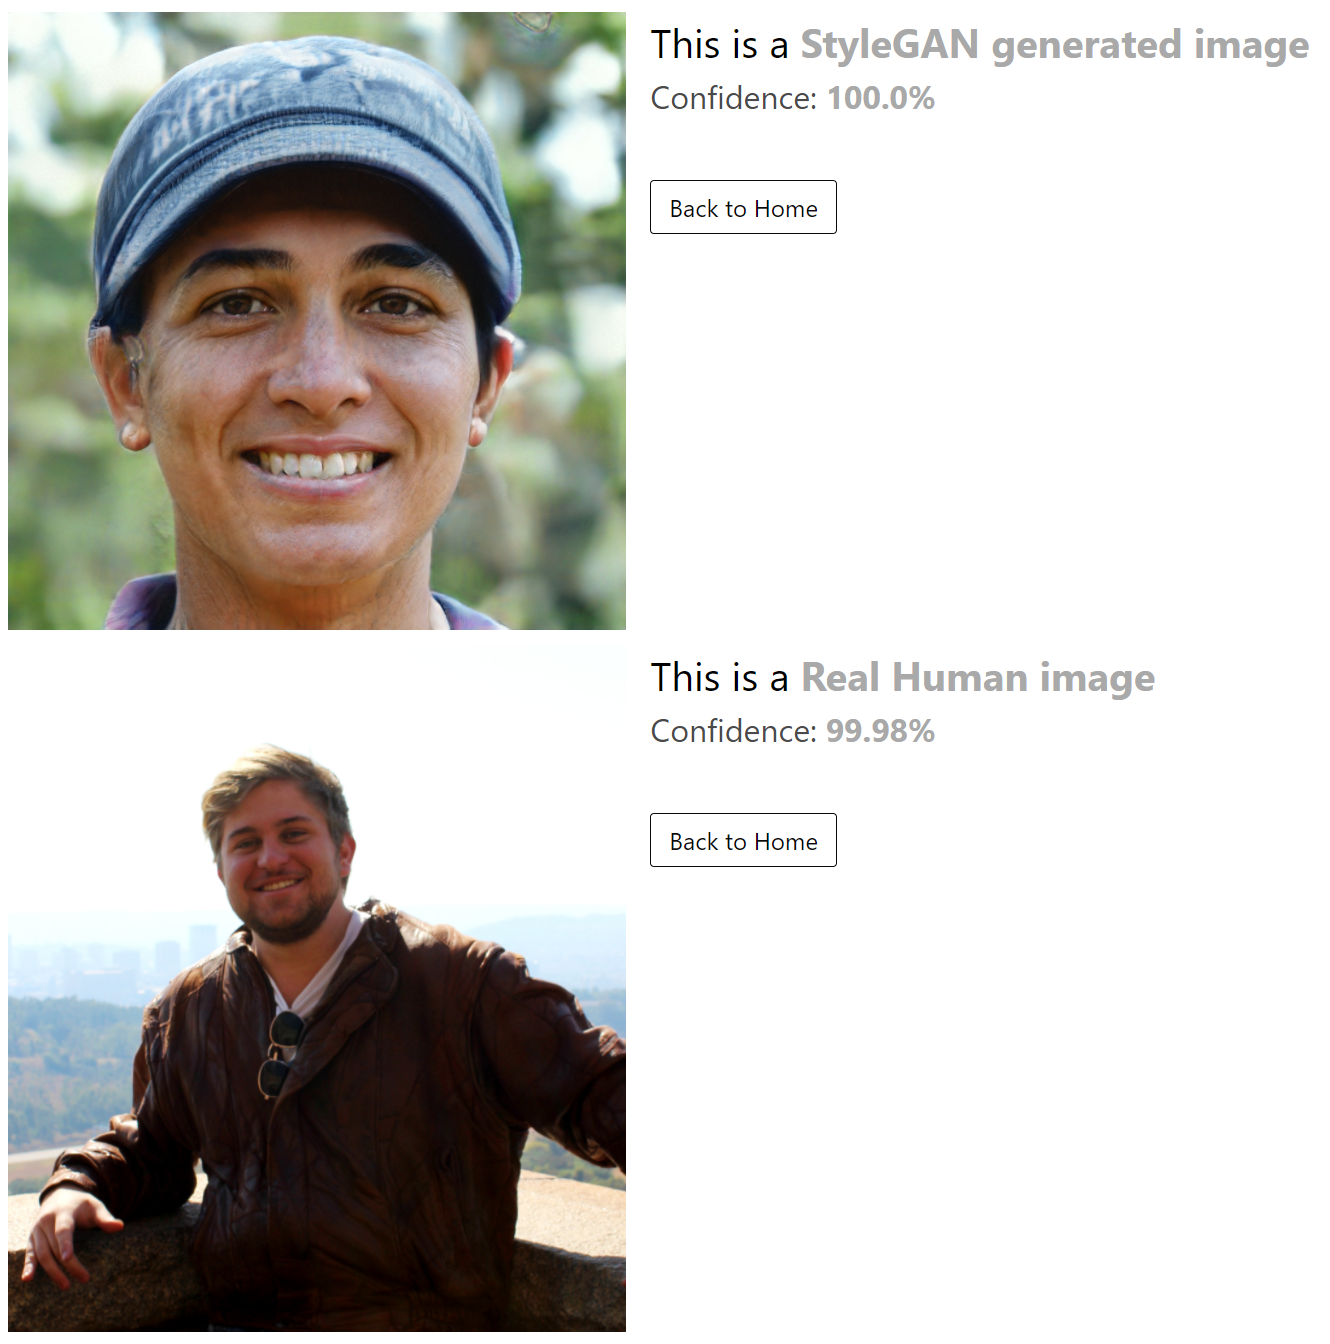
\includegraphics[width=0.85\textwidth]{img/fcomp.png}}%
\caption{Optimized model high confidence and correct prediction}%
\label{fig:rescomp}%
\end{figure}

The optimized model that was created as the final neural network model for this proposed project can identify StyleGAN images and Real human images with high accuracy. Because of the image augmentation previously mentioned the model is also great at generalizing the data. The generalization enables the model to also correctly predict human images not contained in the FlickrFaces dataset. Generalization present in the model helped in the StyleGAN specific images identification but was not as prominent in aiding the function of detection as with generalization with real images. StyleGAN images all originate from the same datasets and GAN, the differences being the version of StyleGAN generated images.  

The small gains in generalizing features from StyleGAN aided in the detection of StyleGAN1 images with fast gains, but when applying the network model to StyleGAN2 images only a small part of generalization aids in the detection of these images. Figure \ref{fig:sg2} shows the detection of StyleGAN2 images using the model of the artefact.

 The model can predict on the images but with the limited testing conducted the prediction of StyleGAN2 images is lower than that of StyleGAN1. This means that this model when implemented will be able to detect some StyleGAN2 images but proves that implementing the same scope of this proposed project on StyleGAN2 and respectively will create a model that can identify these images. A method that can be followed to allow the model to identify all versions of StyleGAN images can be the creation of a dataset that contains StyleGAN, StyleGAN2 and StyleGAN3 images and train a single model on that dataset.

\begin{figure}[H]%
\centering
\fbox{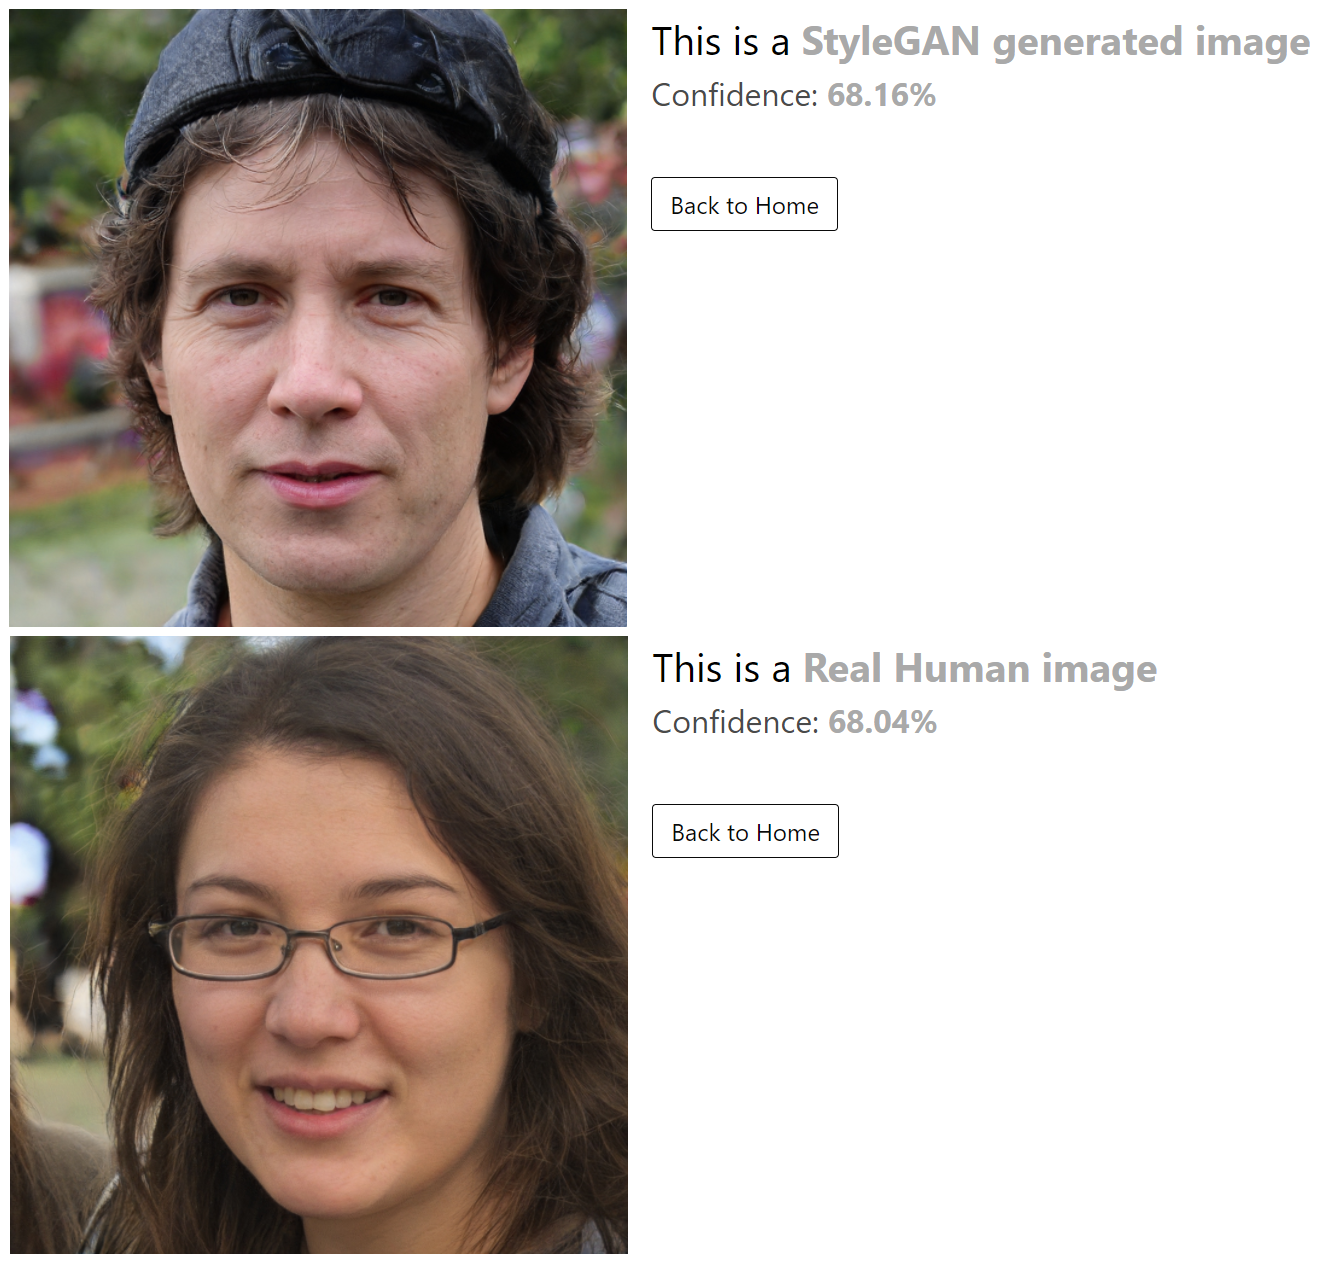
\includegraphics[width=0.85\textwidth]{img/stylegan2.png}}%
\caption{StyleGAN2 tested on the Artefact}%
\label{fig:sg2}%
\end{figure}

The relatively low confidence in Figure \ref{fig:sg2} is a result of the increase in difficulty in detecting StyleGAN2 images. The low confidence also shows that the model is optimized towards the detection of StyleGAN1 images without overfitting. Thus the possibility of a neural network that can detect all three versions of StyleGAN images is proven and can be created similar to the network created by \cite{Wang} but by implementing hyperparameter optimization and reducing the resource needs when creating the model.

\section{Summary}

The result presented by the CNN of the artefact proves the capabilities of Hyperparameter optimization, specifically to Optuna and Binary image classification. The model created in the development of the artefact using hot and cold learning, the simplest approach, showed the performance of CNN's when training models on image datasets. The initial accuracy of the 1\textsuperscript{st} model was relatively high and could be used but the final model's accuracy improved to such an excellent accuracy that it can be used in practice. The scope aim of the project was successfully achieved when analysing the performance of the final model in the detection of StyleGAN images.
